The Atomistic Machine-learning Package (AMP) 
\parencite[Khorshidi, Alizera and Peterson, Andrew A.]{khorshidi2016amp}
is a software package
written in Python with the intent of bringing machine learning
to electronic structure calculations. The software is intended
to interface with ASE and the OpenKIM API for usage
in LAMMPS. The interface to AMP is written purely in Python
while computationally intensive tasks are outsourced to Fortran
modules and the machine learning performed through a Tensorflow
backend. The Python interface makes AMP flexible and easily
extended, and this makes the package ideal for prototyping
and testing both newer and more established machine learning
methods.
\par
A suggested workflow is as follows:

\begin{itemize}
    \item Use AMP for training, testing and validation
        of novel descriptors and systems
    \item Use the AMP calculator for smaller scale
        simulation in the ASE environment
    \item Export the network compliant with the OpenKIM
        API for usage in more mature, large-scale
        electronic structure calculations such as LAMMPS
\end{itemize}

Unfortunately, the software is not currently fully compliant
with the latest version of the OpenKIM API,
which introduces artifacts in the simulation.
However, the authors have recently received a large grant
from the U.S. Department of Energy\footnote{\url{
https://www.brown.edu/news/2018-09-20/simulations}}, 
which should facilitate further development.

\subsection{Theory}
AMP is intended to interface extensively with ASE,
and the primary interface to AMP is the AMP calculator.
The AMP calculator is an ASE compliant calculator
that accepts cartesian coordinates and outputs energies
and forces, just as a classical molecular dynamics calculator.
The primary difference between the AMP calculator
and ASE calculators such as the Lennard-Jones calculator
is the train method, which takes a set of \textit{images}, i.e.
a set of snapshots of atomic configurations labeled
with the potential energy and forces.
The calculator is fitted to the images and can subsequently
used to predict atomic energies and forces from never before seen
atomic configurations.

\begin{figure}[h]
\centering
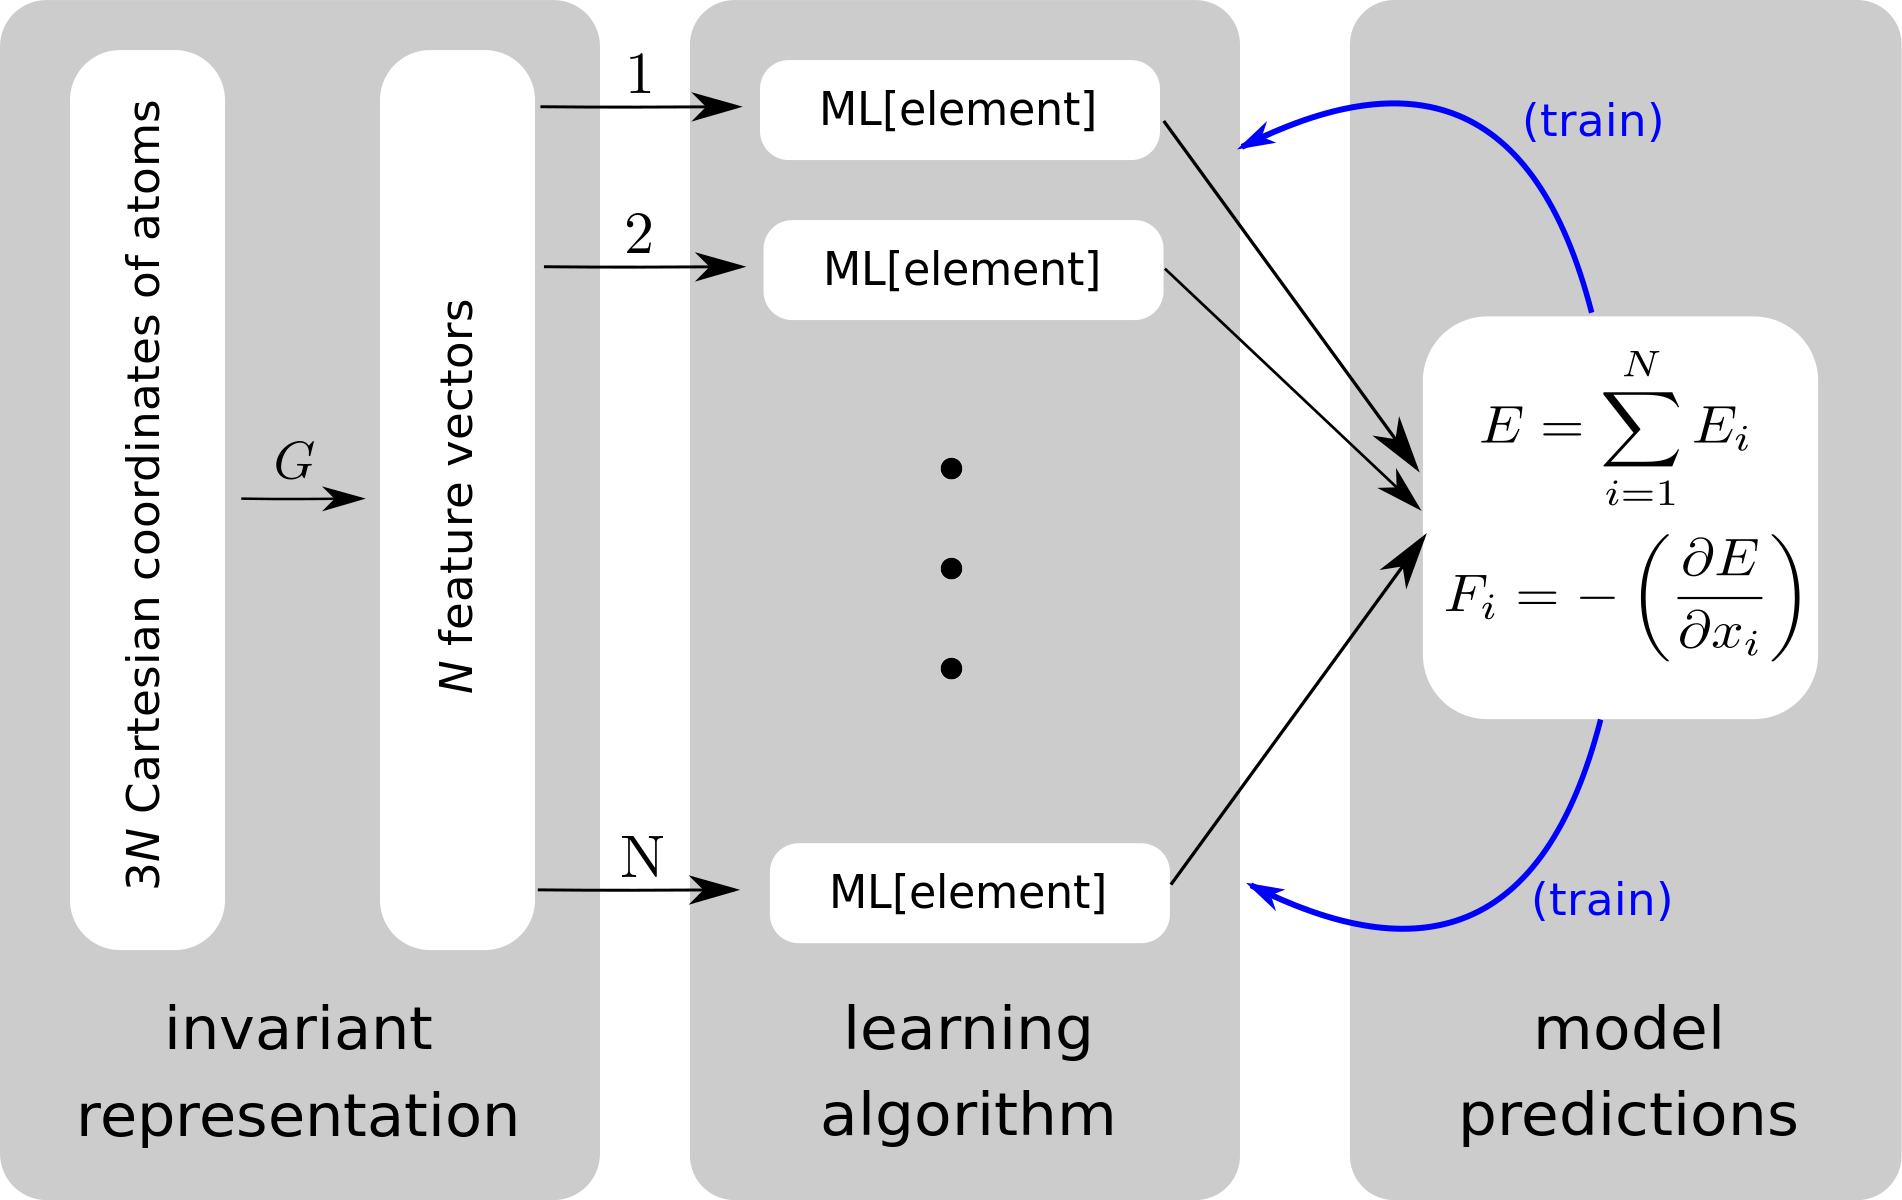
\includegraphics[width=\linewidth]{scheme.png}
\caption{Schematics of how AMP works in atom-centered mode.
    Reprinted from {article}.}
\label{fig:scheme}
\end{figure}

AMP provides interfaces for both atom-centered descriptors, as we
discussed in chapter 6, and image-centered descriptors,
which are formed from the complete set of cartesian coordinates.
A set of feature vectors are formed from an image, which are fed
through a neural network to produce the potential energy.
The neural network is implemented through a Tensorflow interface,
which provides a full neural network graph with weights and
activations. The inputs can be backpropagated through the network
to produce both weight updates and derivatives with respect to
the inputs.

\subsection{Installation}
AMP requires an installation of

\begin{itemize}
    \item Python 2.7, 3.4-3.6, 3.6 is recommended
    \item Numpy 1.9 or newer
    \item Scipy 0.14 or newer
    \item ASE
\end{itemize}

Python installations can be easily obtained through the Anaconda 
or Miniconda packages\footnote{\url{https://anaconda.org/}},
or follow the instructions on the Python website\footnote{
\url{https://www.python.org/}}.
ASE installation is described in the chapter on ASE.
Once you have the prerequisites AMP can be installed using pip:

\begin{lstlisting}[language=bash]
pip install amp-atomistics
\end{lstlisting}

\subsection{Training example}
In the previous chapter we showed how to run a molecular dynamics
simulation using ASE. Here we will show how an AMP calculator
can be fitted to molecular dynamics data with only minor
modifications to the code.
\par
First we import the prerequisites and define the system:

\begin{lstlisting}[language=python,basicstyle=\small]
import ase.io
from ase.lattice.cubic import FaceCenteredCubic
from ase import units
from ase.md.velocitydistribution import MaxwellBoltzmannDistribution
from ase.md.verlet import VelocityVerlet

from amp import AMP
from amp.descriptor.gaussian import Gaussian
from amp.model.neuralnetwork import NeuralNetwork
from amp.model import LossFunction

symbol = "Ar"
size = (3, 3, 3)
atoms = FaceCenteredCubic(symbol=symbol, size=size, pbc=True)
MaxwellBoltzmannDistribution(atoms, 300 * units.kB)
\end{lstlisting}

The class AMP is the primary object of the AMP package,
and is implemented through the ASE interface.
We will use a neural network machine learning model
and Gaussian descriptors, which are an implementation of the
Behler-Parrinello method. To implement force training we require
access to the LossFunction class.
We will also be using the ASE Input/Output (ase.io) module to generate an
ASE \textit{Trajectory}, which is an object
storing the time-evolution of a simulation and usually interpreted
as a time series of atoms.

\begin{lstlisting}
traj = ase.io.Trajectory("training.traj", "w")
calc = LennardJones(sigma=3.405, epsilon=1.0318e-2)
atoms.set_calculator(calc)
atoms.get_potential_energy()
atoms.get_forces()
dyn = VelocityVerlet(atoms, 5 * units.fs)
traj.write(atoms)
\end{lstlisting}

In order to write the potential energy and forces to file
they must first be calculated using the ASE Atoms methods,
which require a calculator and otherwise raise an error.
We can then evolve the system forward in time
and save the atomic configuration every 10 time steps:

\begin{lstlisting}
for i in range(100):
    dyn.run(10)
    atoms.get_potential_energy()
    atoms.get_forces()
    traj.write(atoms)
\end{lstlisting}

After the data has been generated we can train the AMP calculator
using the Lennard-Jones calculations as input:

\begin{lstlisting}
calc = Amp(descriptor=Gaussian(),
           model=NeuralNetwork(hiddenlayers=(10, 10, 10)))
calc.model.lossfunction = LossFunction(
           convergence={"energy_rmse": 1E-2,
                        "force_rmse": 1E-2})
calc.train(images="training.traj")
\end{lstlisting}

Once the calculator has been trained, the parameters
are stored in a file called "amp.amp",
and can be loaded using the command:

\begin{lstlisting}
calc = Amp.load("amp.amp")
\end{lstlisting}

From there the calculator can be used as any other ASE calculator,
in electronic structure calculations on Atoms objects.

\subsection{Descriptors}
Currently AMP provides support for three different descriptors.
Gaussian descriptors implement the Behler-Parrinello method
of radial and angular symmetry functions. For this descriptor
the derivatives are also available, which means it can be used
for computing dynamics. Some physical intuition and chemical knowledge
is necessary to choose various parameters for the symmetry functions -
unless you wish to do it by trial and error - but AMP provides
defaults for multiple chemical species.
\par
Zernike descriptors represent a tensor product between spherical
harmonics and Zernike polynomials. The local atomic environment
of atom $i$is represented by an atomic density function $\rho_i(\bm{r}_i)$:

\begin{equation}
 \rho_i(\bm{r}_i) = \sum_{j\neq i}^{\text{local}}
    \eta_j \delta \left( \bm{r}_i - \bm{r}_{ij} \right)
    f_c \left( \lvert \lvert \bm{r}_{ij} \rvert \rvert \right) , 
\end{equation}

with $f_c(r)$ a cutoff function as described in chapter 6.
The 3-D Zernike basis set $Z$ is formed by a tensor product between
the Zernike polynomials basis set $R$ and the spherical harmonics
$Y$. The Zernike basis set is defined inside and on the surface
of the $S^2$ unit sphere as:

\begin{equation}
 Z_{nl}^m (r, \theta, \phi) = R_n^l(r) Y_l^m(\theta, \phi) , 
\end{equation}

where $n \geq 0$ is an integer, $l$ is restricted to even $n - l \geq 0$
and $m$ is an integer such that $\left| m \right| \leq l$.
Functions defined inside and on the $S^2$ sphere
can be represented by the 3-D Zernike basis as:

\begin{equation}
 f(r, \theta, \phi) = \sum_{n=0}^{\infty} \sum_l \sum_{m=-l}^l
    c_{nl}^m Z_{nl}^m (r, \theta, \phi) , 
\end{equation}

with coefficients $c_{nl}^m = \langle Z_{nl}^m, f \rangle$
computed as projections of $f$ onto the Zernike basis.
These projections form the basis of the Zernike fingerprint,
$\bm{G}_i$. Centering the atomic density preserves translation
invariance of the atomic environment, while the projections
onto the Zernike basis set preserves rotational invariance.
Permutation invariance is maintained by keeping the constant values
$\eta_j$ the same within each chemical species.
\par
Bispectrum descriptors are computed much in the same way
as the Zernike descriptors. The 4-D spherical harmonics
form a complete, orthogonal basis set for the $S^3$ 4-D unit
sphere, and the components of the Bispectrum fingerprints
$\bm{G}_i$ can be computed by projecting the atomic
density function onto them. For more information
the reader is encouraged to check out the AMP paper [ref here].
